% Copyright (c) 2026 CorrectBrain
% SPDX-License-Identifier: MIT

\PassOptionsToPackage{dvipsnames,svgnames,x11names}{xcolor}
\documentclass[tikz,border=8pt]{standalone}
\usetikzlibrary{arrows.meta,positioning,calc,shapes,shadows,decorations.pathmorphing,shapes.geometric,backgrounds,decorations.markings,decorations.pathreplacing,decorations.text,fit,shapes.misc,shapes.arrows,matrix,bending,3d,chains,intersections,shapes.symbols,svg.path,shapes.multipart,snakes,shapes.callouts,angles,quotes}
\providecolor{gold}{RGB}{212,175,55}
\providecolor{silver}{RGB}{192,192,192}
\providecolor{bronze}{RGB}{205,127,50}
\providecolor{darkblue}{RGB}{0,0,139}
\providecolor{lightblue}{RGB}{173,216,230}
\providecolor{darkgreen}{RGB}{0,100,0}
\providecolor{lightgreen}{RGB}{144,238,144}
\providecolor{darkred}{RGB}{139,0,0}
\providecolor{navy}{RGB}{0,0,128}
\providecolor{skyblue}{RGB}{135,206,235}
\providecolor{beige}{RGB}{245,245,220}
\providecolor{cream}{RGB}{255,253,208}
\usepackage{amsmath}
\usepackage{amssymb}
\usepackage{fontawesome5}
\usetikzlibrary{fadings,shadows.blur,patterns,patterns.meta}

\providecolor{gold}{RGB}{212,175,55}
\providecolor{silver}{RGB}{192,192,192}
\providecolor{bronze}{RGB}{205,127,50}
\providecolor{darkblue}{RGB}{0,0,139}
\providecolor{lightblue}{RGB}{173,216,230}
\providecolor{darkgreen}{RGB}{0,100,0}
\providecolor{lightgreen}{RGB}{144,238,144}
\providecolor{darkred}{RGB}{139,0,0}
\providecolor{navy}{RGB}{0,0,128}
\providecolor{skyblue}{RGB}{135,206,235}
\providecolor{beige}{RGB}{245,245,220}
\providecolor{cream}{RGB}{255,253,208}
\usepackage{amsmath}
\usepackage{amssymb}
\usepackage{fontawesome5}


\usepackage{tikz}
\usepackage{xcolor}

% --- DEFINE THEMATIC PALETTE ---
\definecolor{browserbg}{HTML}{F8F9FA}
\definecolor{browserchrome}{HTML}{E9ECEF}
\definecolor{legacyred}{HTML}{E74C3C}
\definecolor{moderngreen}{HTML}{27AE60}
\definecolor{enginepurple}{HTML}{8E44AD}
\definecolor{darkgray}{HTML}{2C3E50}
\definecolor{textgray}{HTML}{7F8C8D}
\definecolor{dotred}{HTML}{FF5F56}
\definecolor{dotyellow}{HTML}{FFBD2E}
\definecolor{dotgreen}{HTML}{27C93F}

\begin{document}
\begin{tikzpicture}[
    every node/.style={font=\sffamily},
    browserwin/.style={
        fill=browserbg,
        draw=gray!30,
        thick,
        rounded corners=4pt,
        drop shadow={shadow xshift=0ex, shadow yshift=-0.5ex, opacity=0.15}
    },
    conclusioncard/.style={
        fill=white,
        draw=gray!30,
        rounded corners=6pt,
        inner sep=15pt,
        text width=11cm,
        drop shadow={shadow xshift=0ex, shadow yshift=-1ex, opacity=0.1}
    }
]

% --- CANVAS BOUNDING BOX ENFORCEMENT ---
\path[fill=white] (-16, 17.0) rectangle (16, -11);

% ==========================================
% GLOBAL TITLES & HEADINGS
% ==========================================
\node[font=\Huge\bfseries\color{darkgray}, text width=26cm, align=center] at (0.0248,16.9451) {Temporal Layout Mechanics \& CLS Mitigation};
\node[font=\Large\color{gray}, text width=22cm, align=center] at (0.0248,15.9451) {How \texttt{aspect-ratio} preempts layout thrashing chronologically during the render pipeline};


% ==========================================
% RENDER PIPELINE PILLAR (TIMELINE)
% ==========================================
% Timeline 3D structural pipe with shaded gradient look
\draw[line width=8pt, line cap=round, draw=gray!40, -Stealth=3mm] (0, 14.0) -- (0, -6.5);
\node[font=\bfseries\sffamily\color{darkgray}, fill=white, inner sep=4pt, rounded corners=2pt, draw=gray!20] at (0, 14.3) {TIME (Render Pipeline)};

% Time Marker t1
\fill[enginepurple, opacity=0.3] (0, 12.0) circle (12pt);
\fill[enginepurple] (0, 12.0) circle (5pt);
\fill[white] (0, 12.0) circle (2pt);
\node[anchor=center, text width=7cm, align=center, font=\large\bfseries\color{enginepurple}, fill=white, inner sep=4pt, rounded corners=3pt, drop shadow={shadow xshift=0ex, shadow yshift=-0.2ex, opacity=0.1}] at (0, 11.4) {$t_1$: Initial DOM Parse (CSSOM Constructed)};

% Time Marker t2
\fill[enginepurple, opacity=0.3] (0, 3.0) circle (12pt);
\fill[enginepurple] (0, 3.0) circle (5pt);
\fill[white] (0, 3.0) circle (2pt);
\node[anchor=center, text width=7cm, align=center, font=\large\bfseries\color{enginepurple}, fill=white, inner sep=4pt, rounded corners=3pt, drop shadow={shadow xshift=0ex, shadow yshift=-0.2ex, opacity=0.1}] at (0, 2.2) {$t_2$: Image Payload Resolved (Network Request Complete)};


% ==========================================
% LEFT SIDE: LEGACY (UNCONSTRAINED MEDIA)
% ==========================================
\node[font=\huge\bfseries\color{legacyred}, text width=12cm, align=center] at (-7.5, 13.6) {Legacy: Unconstrained Media};
\node[font=\large\color{gray}, text width=12cm, align=center] at (-7.5, 12.6) {\texttt{width: 100\%;} (No explicit ratio)};

% --- t1 Left: Layout Unknown ---
\node[font=\bfseries\color{legacyred}, text width=6cm, align=center] at (-7, 10.0) {Layout Engine: ``Unknown block-size. Reserving 0px.''};

% Browser Window 1 (t1)
\path[browserwin] (-10, 3.5) rectangle (-4, 9.0);
% Chrome Header (squared-off bottom)
\path[fill=browserchrome, rounded corners=4pt] (-10, 8.6) rectangle (-4, 9.0);
\path[fill=browserchrome] (-10, 8.6) rectangle (-4, 8.8);
% Mac-style Chrome Dots
\fill[dotred] (-9.6, 8.8) circle (3pt);
\fill[dotyellow] (-9.3, 8.8) circle (3pt);
\fill[dotgreen] (-9.0, 8.8) circle (3pt);

% Image Box: 0 Height Line
\draw[dashed, legacyred, very thick] (-9.5, 8.2) -- (-4.5, 8.2);
\node[font=\tiny\bfseries\color{legacyred}] at (-7, 8.45) {\faExclamationTriangle \quad Zero Height};

% Document Flow (Text Blocks)
\filldraw[gray!40, draw=none, rounded corners=1pt] (-9.5, 7.8) rectangle (-4.5, 7.5);
\filldraw[gray!40, draw=none, rounded corners=1pt] (-9.5, 7.3) rectangle (-6.0, 7.0);
\node[font=\small\bfseries\color{darkgray}, text width=5.5cm, align=center] at (-7, 6.2) {Following document flow is rendered artificially high.};


% --- t2 Left: Post Layout Shift ---
\node[font=\bfseries\color{legacyred}, text width=6cm, align=center] at (-7, 0.8) {Layout Engine: ``Image loaded. Recalculating Document!''};

% Browser Window 2 (t2)
\path[browserwin] (-10, -6.0) rectangle (-4, -0.5);
% Chrome Header (squared-off bottom)
\path[fill=browserchrome, rounded corners=4pt] (-10, -0.9) rectangle (-4, -0.5);
\path[fill=browserchrome] (-10, -0.9) rectangle (-4, -0.7);
% Mac-style Chrome Dots
\fill[dotred] (-9.6, -0.7) circle (3pt);
\fill[dotyellow] (-9.3, -0.7) circle (3pt);
\fill[dotgreen] (-9.0, -0.7) circle (3pt);

% Image Box: Exact 16:9 Calculated Dimensions (Width=5, Height=2.8125, Y: -1.3 to -4.1125)
\begin{scope}
    \clip[rounded corners=2pt] (-9.5, -1.3) rectangle (-4.5, -4.1125);
    \fill[legacyred!12] (-9.5, -1.3) rectangle (-4.5, -4.1125);
    % Stylized vector landscape (red/gray tones pushed down)
    \fill[legacyred!25] (-8.6, -3.0) circle (0.25);
    \fill[legacyred!35] (-9.5, -4.1125) -- (-8.2, -2.8) -- (-6.9, -4.1125) -- cycle;
    \fill[legacyred!20] (-7.7, -4.1125) -- (-6.3, -2.85) -- (-4.5, -4.1125) -- cycle;
    \fill[legacyred!45] (-9.5, -4.1125) .. controls (-8.0, -3.3) and (-6.0, -3.8) .. (-4.5, -4.1125) -- cycle;
\end{scope}
\draw[legacyred, thick, rounded corners=2pt] (-9.5, -1.3) rectangle (-4.5, -4.1125);
\node[font=\large\bfseries\color{legacyred!90!black}, fill=white, fill opacity=0.88, text opacity=1, rounded corners=3pt, inner sep=3pt] at (-7, -2.70625) {\faImage \quad Media Loaded};

% Shifted Text Blocks (Moved down by exactly 2.8125 units)
\filldraw[gray!40, draw=none, rounded corners=1pt] (-9.5, -4.5125) rectangle (-4.5, -4.8125);
\filldraw[gray!40, draw=none, rounded corners=1pt] (-9.5, -5.0125) rectangle (-6.0, -5.3125);

% Cumulative Layout Shift (CLS) Indicator & Arrow
\draw[-Stealth=3mm, line width=3pt, legacyred] (-10.5, -1.7) -- (-10.5, -4.5125);
\node[anchor=east, align=center, font=\bfseries\color{legacyred}, fill=white, inner sep=6pt, draw=legacyred, rounded corners=3pt, drop shadow={shadow xshift=0ex, shadow yshift=-0.2ex, opacity=0.1}] at (-11.0, -3.1) {CUMULATIVE LAYOUT SHIFT (CLS)\\[4pt] \textbf{CLS: 2.8125 units}};


% ==========================================
% RIGHT SIDE: MODERN (aspect-ratio: 16/9)
% ==========================================
\node[font=\huge\bfseries\color{moderngreen}, text width=12cm, align=center] at (7.5, 13.6) {Modern: \texttt{aspect-ratio: 16/9}};
\node[font=\large\color{gray}, text width=12cm, align=center] at (7.5, 12.6) {Algorithmic Intrinsic Sizing};

% --- t1 Right: Layout Pre-allocated ---
\node[font=\bfseries\color{moderngreen}, text width=6.5cm, align=center] at (7, 10.0) {Layout Engine: ``Solving $H = W \times \frac{9}{16}$. Reserving exact space.''};

% Browser Window 3 (t1)
\path[browserwin] (4, 3.5) rectangle (10, 9.0);
% Chrome Header (squared-off bottom)
\path[fill=browserchrome, rounded corners=4pt] (4, 8.6) rectangle (10, 9.0);
\path[fill=browserchrome] (4, 8.6) rectangle (10, 8.8);
% Mac-style Chrome Dots
\fill[dotred] (4.4, 8.8) circle (3pt);
\fill[dotyellow] (4.7, 8.8) circle (3pt);
\fill[dotgreen] (5.0, 8.8) circle (3pt);

% Pre-allocated Image Box (Width=5, Height=2.8125, Y: 8.2 to 5.3875)
\draw[dashed, moderngreen, very thick, fill=moderngreen!5, pattern=north west lines, pattern color=moderngreen!20] (4.5, 8.2) rectangle (9.5, 5.3875);
\node[font=\large\bfseries\color{moderngreen}, fill=white, fill opacity=0.9, text opacity=1, rounded corners=3pt, inner sep=3pt] at (7, 6.79375) {\faHourglassHalf \quad Space Pre-allocated};
\draw[{Stealth[length=5pt]}-Stealth=3mm, moderngreen, thick] (10.4, 8.2) -- (10.4, 5.3875) node[midway, right, font=\footnotesize\bfseries\color{moderngreen}] {Computed $H$};

% Document Flow (Rendered in Final Position)
\filldraw[gray!40, draw=none, rounded corners=1pt] (4.5, 4.9875) rectangle (9.5, 4.6875);
\filldraw[gray!40, draw=none, rounded corners=1pt] (4.5, 4.4875) rectangle (6.0, 4.1875);


% --- t2 Right: Zero Layout Shift ---
\node[font=\bfseries\color{moderngreen}, text width=6.5cm, align=center] at (7, 0.8) {Layout Engine: ``Image loaded. Plotting into pre-allocated buffer.''};

% Browser Window 4 (t2)
\path[browserwin] (4, -6.0) rectangle (10, -0.5);
% Chrome Header (squared-off bottom)
\path[fill=browserchrome, rounded corners=4pt] (4, -0.9) rectangle (10, -0.5);
\path[fill=browserchrome] (4, -0.9) rectangle (10, -0.7);
% Mac-style Chrome Dots
\fill[dotred] (4.4, -0.7) circle (3pt);
\fill[dotyellow] (4.7, -0.7) circle (3pt);
\fill[dotgreen] (5.0, -0.7) circle (3pt);

% Image Box: Media Loaded into Buffer (Exact match Y: -1.3 to -4.1125)
\begin{scope}
    \clip[rounded corners=2pt] (4.5, -1.3) rectangle (9.5, -4.1125);
    \fill[moderngreen!12] (4.5, -1.3) rectangle (9.5, -4.1125);
    % Stylized vector landscape (green tones)
    \fill[moderngreen!25] (5.4, -1.9) circle (0.35);
    \fill[moderngreen!35] (4.5, -4.1125) -- (5.8, -2.5) -- (7.1, -4.1125) -- cycle;
    \fill[moderngreen!20] (6.3, -4.1125) -- (7.7, -2.1) -- (9.5, -4.1125) -- cycle;
    \fill[moderngreen!45] (4.5, -4.1125) .. controls (6.0, -3.3) and (8.0, -3.8) .. (9.5, -4.1125) -- cycle;
\end{scope}
\draw[moderngreen, thick, rounded corners=2pt] (4.5, -1.3) rectangle (9.5, -4.1125);
\node[font=\large\bfseries\color{moderngreen!90!black}, fill=white, fill opacity=0.88, text opacity=1, rounded corners=3pt, inner sep=3pt] at (7, -2.70625) {\faImage \quad Media Loaded};

% Document Flow (Unmoved relative to viewport)
\filldraw[gray!40, draw=none, rounded corners=1pt] (4.5, -4.5125) rectangle (9.5, -4.8125);
\filldraw[gray!40, draw=none, rounded corners=1pt] (4.5, -5.0125) rectangle (6.0, -5.3125);

% Zero Layout Shift Indicator (Exterior Alignment Line)
\draw[dashed, moderngreen, line width=1.5pt] (10.3, 4.9875) -- (10.3, -4.5125);
\node[anchor=west, align=center, font=\bfseries\color{moderngreen}, fill=white, inner sep=5pt, draw=moderngreen, rounded corners=4pt, drop shadow={shadow xshift=0ex, shadow yshift=-0.3ex, opacity=0.1}] at (10.7, 0.2375) {\faCheckCircle \quad ZERO LAYOUT SHIFT\\[4pt] (Alignment Maintained)};


% ==========================================
% BOTTOM CONCLUSION PANELS
% ==========================================
% Left Panel (Legacy)
\node[anchor=north, conclusioncard, text width=11cm] at (-7, -7.5) {
    {\large\bfseries\color{legacyred}\faExclamationTriangle \quad Layout Thrashing}\\[6pt]
    {\normalsize\color{darkgray} Without \texttt{aspect-ratio}, the browser cannot mathematically derive the height until the physical file's headers arrive over the network. It defers layout space (0px). When the payload finally arrives, it forces a computationally expensive geometry recalculation of the entire document tree, shifting all subsequent nodes and jarring the user.}
};

% Right Panel (Modern)
\node[anchor=north, conclusioncard, text width=11cm] at (7, -7.5) {
    {\large\bfseries\color{moderngreen}\faCheckCircle \quad Preemptive Geometric Resolution}\\[6pt]
    {\normalsize\color{darkgray} The \texttt{aspect-ratio} specification acts as a declarative mathematical constraint. The layout engine computes the target bounding box instantly during the initial CSSOM render tree construction. The physical bytes of the image are strictly decoupled from the DOM geometry.}
};

\end{tikzpicture}
\end{document}
